\documentclass{article}
\usepackage{amsmath}
\usepackage{hyperref}
\usepackage{amsfonts}
\usepackage{bookmark}
\usepackage{float} 
\usepackage{graphicx}
\usepackage{makeidx}
\usepackage{pgfplots}
\usepackage[letterpaper, total={7.5in, 10in}]{geometry}


\makeindex
\pgfplotsset{compat=1.18}
\begin{document}
\title{Test 1 Prep \\
    \large{Semester 2}}
\author{Elias Xu}
\date{\today}
\maketitle

\tableofcontents

\setlength{\parindent}{0pt}

\section{Introduction}

The topics on the test are: 
\begin{itemize}
    \item Double Integrals in Rectangular and Polar form
    \item Triple Integrals in Rectangular form, Cylindrical and (maybe) Spherical form
    \item Changing the order of integration
\end{itemize}

\section{Double Integrals}

There are two main topics that we have to discuss regarding double integrals: first about rectagular and polar forms

\subsection{Double Integrals in Rectangular Form}

I'll be copying stuff from the last test, cause this section is kinda simple. 


\subsubsection{Fubini's Theorem and Evaluating Double Integrals}

Evaluating double integrals is like counting up loafs of bread, and Fubini's theorem says that no matter how one slices, you'll get the same amount of bread. Y will have to take the slices (integrals over the contours) of either x or y, getting a area function given the other variable, and then integrate that or its range. \\ 
Thus, Fubini's theorem states that if $f(x, y)$ is continious on $[a, b] \times [c, d]$ then $\iint_{R} f(x, y) \delta A$ equals:
\begin{align*}
    V = \int_{a}^{b} B(x) \delta x = \int_{a}^{b} \left[ \int_{c}^{d} f(x,y) \delta y \right] \delta x  &  & B(x) = \int_{c}^{d} f(x, y) \delta x \\
    V = \int_{c}^{d} A(y) \delta y = \int_{c}^{d} \left[ \int_{a}^{b} f(x, y) \delta x \right] \delta y &  & A(y) = \int_{a}^{b} f(x, y) \delta y
\end{align*}


\subsubsection{The Very Nice Theorem}

Interesting way to evauate integrals that can be separated into individual components.
$$\text{If } f(x, y) = g(x)h(y) \text{ and R} = [a, b] \times [c, d] \text{, then} \\ \iint_{R} f(x, y) \delta A = \int_{a}^{b} g(x) \delta x \int_{c}^{d} h(y) \delta y $$

\subsubsection{Double Integral Properties (over Rectangles)}

\begin{itemize}
    \item  $\iint_{R} (f + g) \delta A = \iint_{R} f \delta A + \iint_{R} g \delta A$
    \item $\iint_{R} cf(x,y) \delta A = c \iint_{R} f(x, y) \delta A$
    \item If $f(x, y) \ge g(x, y)$, then $\iint_{R} f(x, y) \delta A \ge \iint_{R} g(x, y)$. (i.e. integrals preserve inequalities)
\end{itemize}

\subsubsection{Evaluating Double Integrals over Non-Rectangular Boundaries}

A big idea relating to evaluating double integrals over non-rectangular boundaries is how to find a bound, because it's more interesting/difficult to do so with these odd bounds. Thus we need to differential between type 1, type 2, and non-typal shapes.

\subsubsection{Type 1 Shapes vs Type 2 Shapes}

\textbf{Type 1 Bound}\\
Type one shapes have a $x \in \lbrack a, b \rbrack$ as boundaries, and are defined by two $y = g(x)$ functions.
\begin{figure}[H]
    \centering
    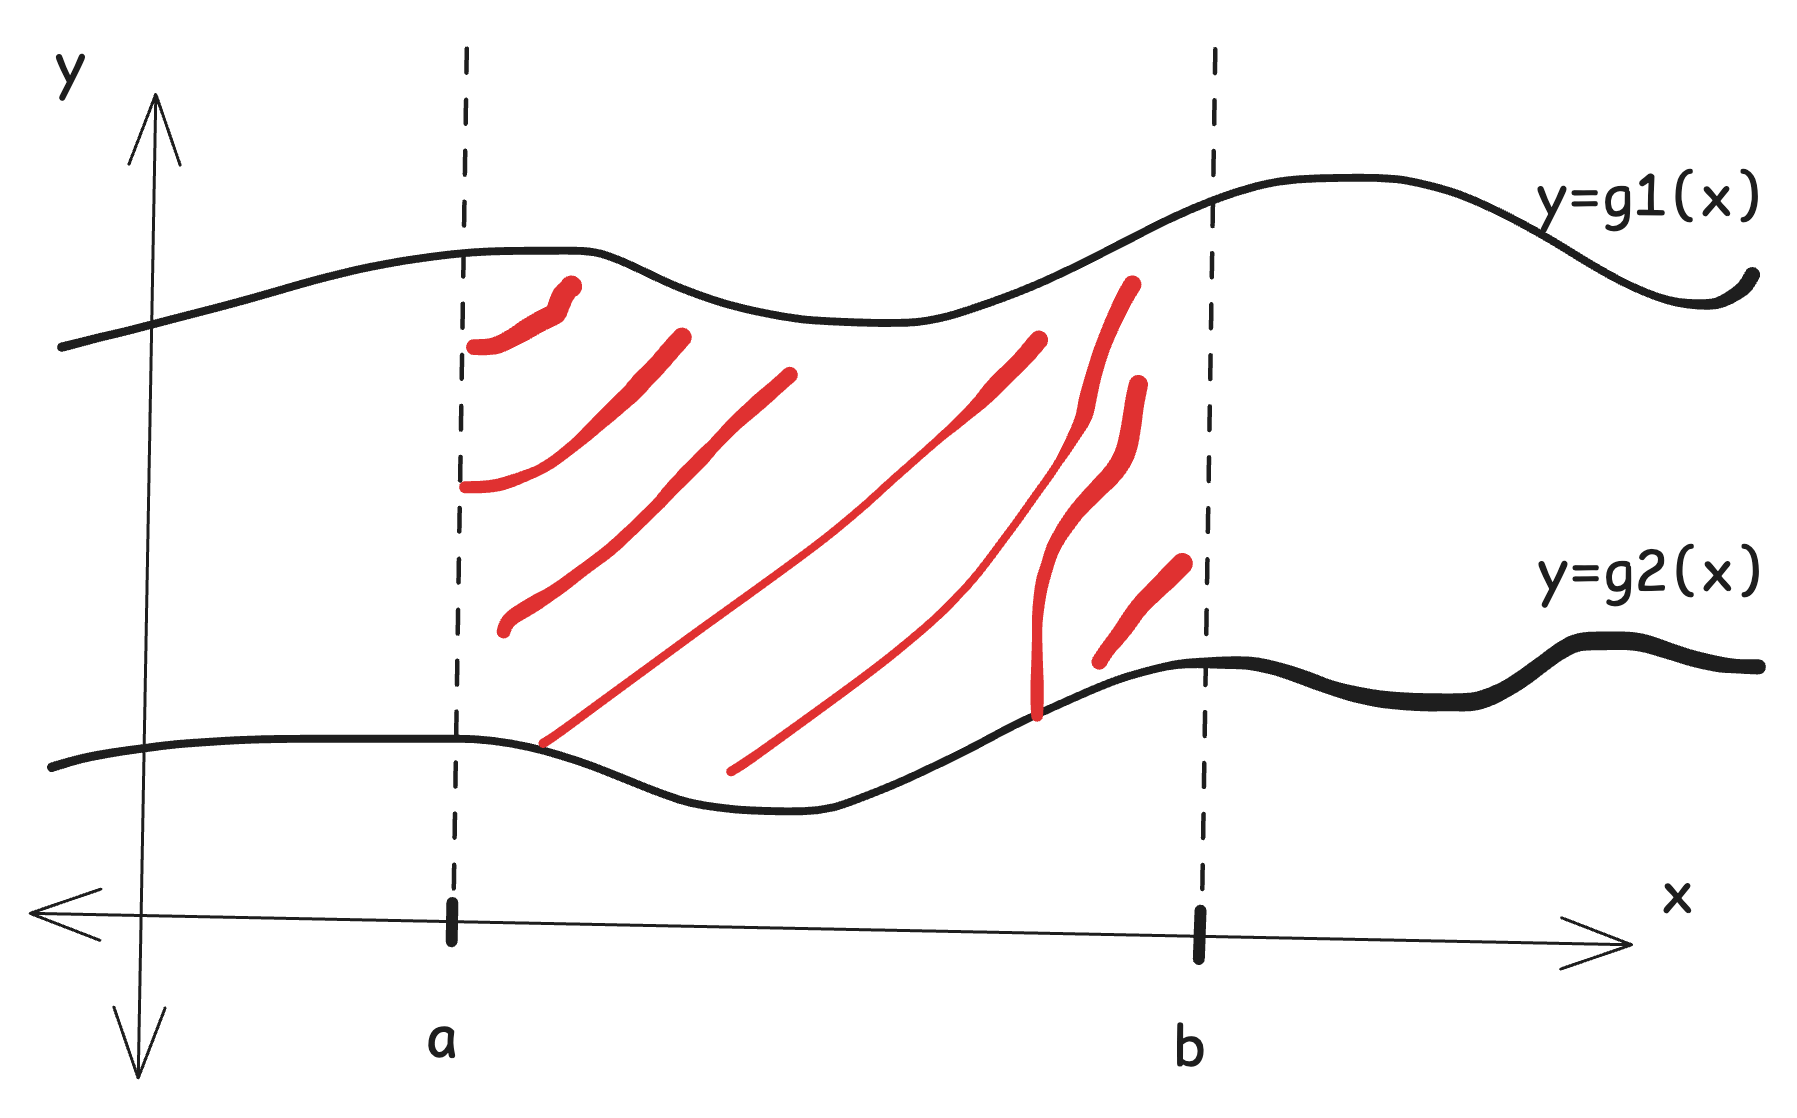
\includegraphics[width=0.5\textwidth]{figures/Type1Example.png}
    \caption{Example of a Type 1 bound}
\end{figure}
\textbf{Type 2 Bound} \\
Type 2 shapes have a $y \in \lbrack a, b \rbrack$ as boundaries, and are defined by two $x = h(y)$ functions
\begin{figure}[H]
    \centering
    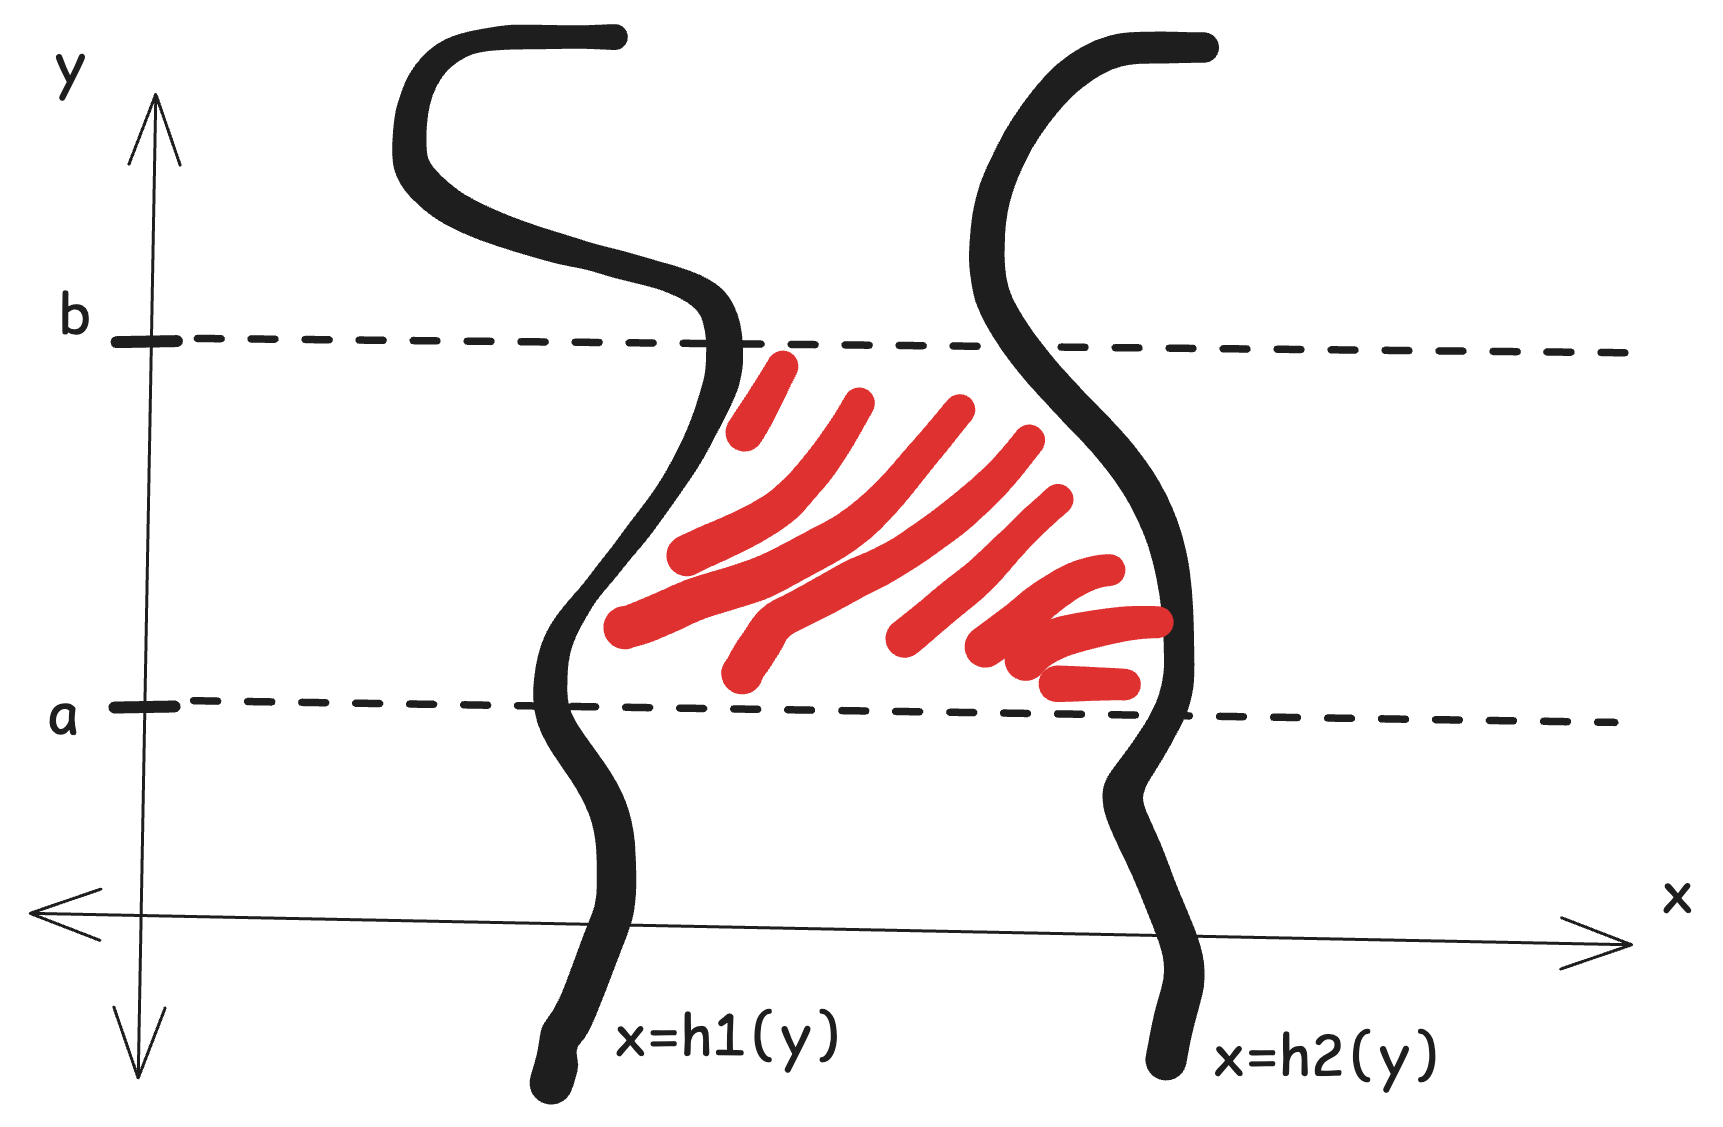
\includegraphics[width=0.5\textwidth]{figures/Type2Example.png}
    \caption{Example of a Type 2 Bound}
\end{figure}
\textbf{NOTE:} There are some surfaces that are BOTH type 1 and type 2 boundaries, such as a circle.

\subsubsection{Integrating over Type 1 and Type 2 Bounds}
There are \emph{TWO OPTIONS}
\begin{itemize}
    \item If the bounds are \textbf{functions of x}, or the base is a \textbf{type 1}, $$V = \iint_D f(x, y) \delta A = \int_{a}^{b} \big[ \int_{g_1(x)}^{g_2(x)} f(x, y) \delta y \big]\delta x$$
    \item If the bounds are \textbf{functions of y}, of the base is a \textbf{type 2}, $$V = \iint_D f(x, y) \delta A =\int_{c}^{d} \big[\int_{h_1(y)}^{h_2(y)} f(x, y) \delta x \big]  \delta y $$
\end{itemize}

\subsubsection{Example}
Find the volume of $z = 8 - 4x - 2y$ over the boundary:
\begin{figure}[H]
    \centering
    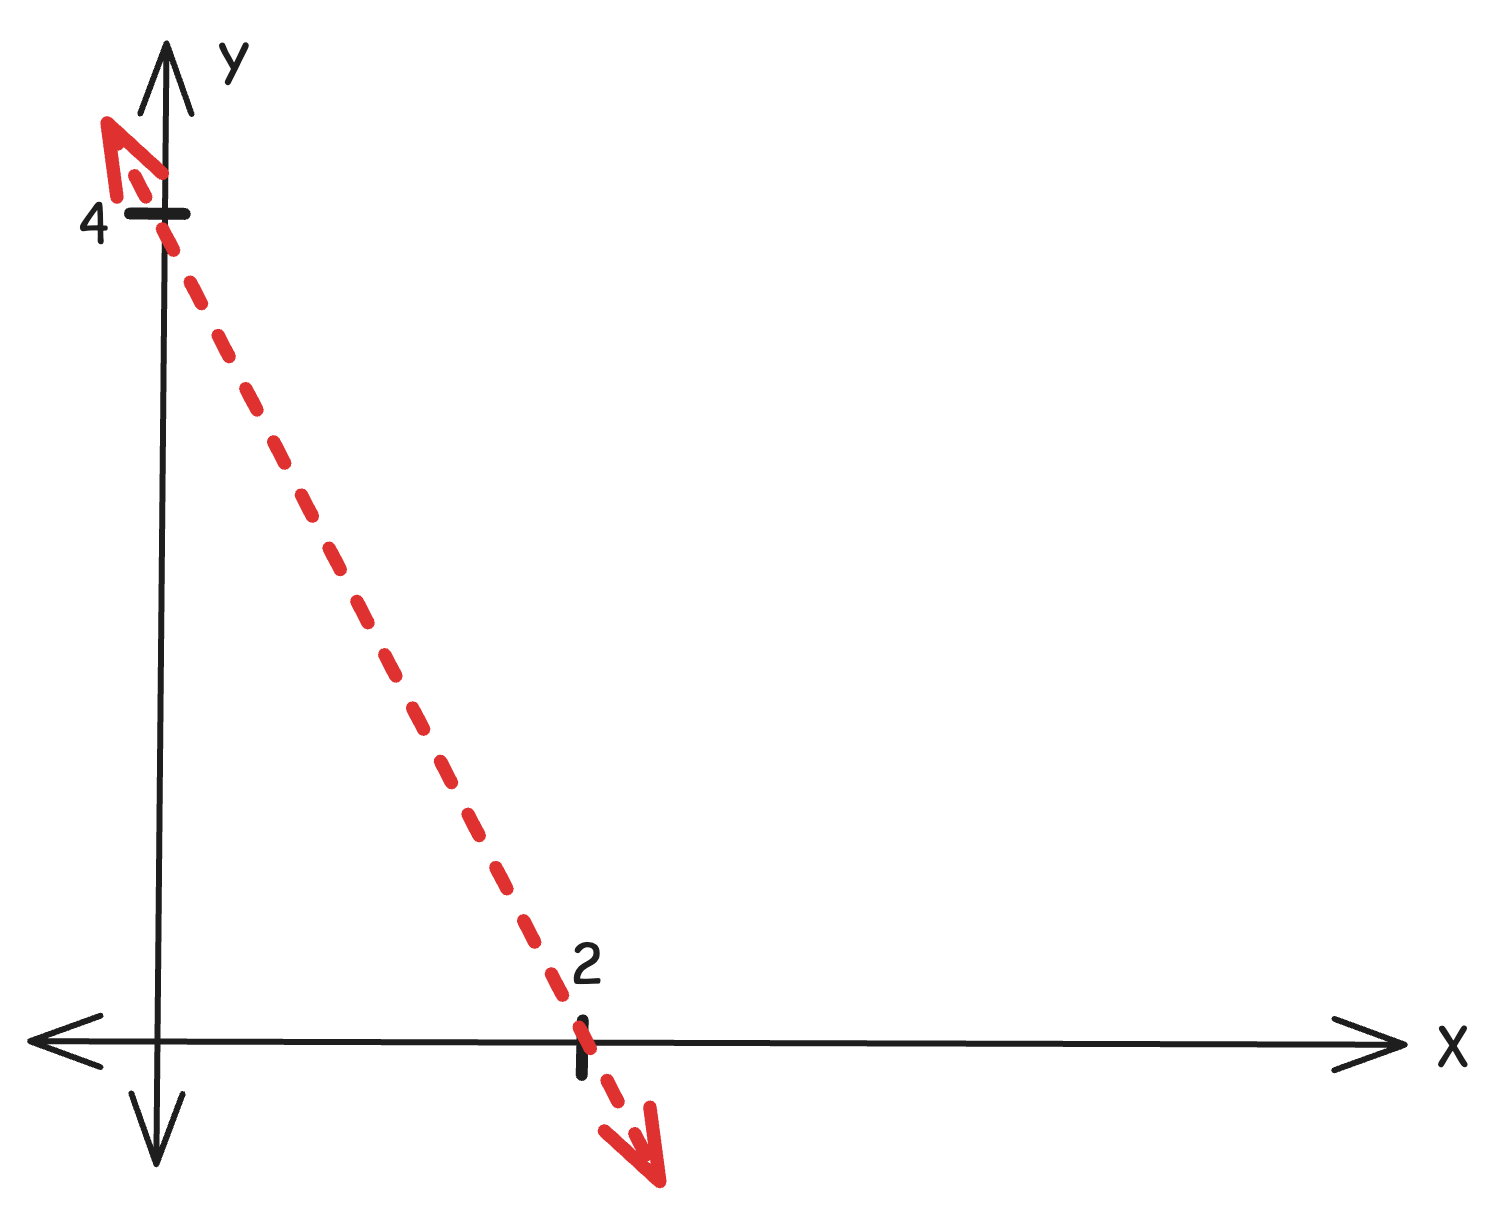
\includegraphics[width=0.3\textwidth]{figures/BoundedExample.png}
\end{figure}
The bound is both a type 1 and a type 2 integral, but let's start with integrating as a type 1 integral.
$$\int_{0}^{2} \big[\int_{0}^{-2x+4} f(x, y) \delta y\big] \delta x$$
$$= \int_{0}^{2} \big[8y - 4xy - y^2\big|_0^{-2x+4}\big] \delta x$$
$$= \int_{0}^{2} \big[8(-2x+4) - 4(x)(-2x+4) - (-2x+4)^2\big] \delta x$$
$$= \int_{0}^{2} 4x^2 - 16 x + 16 \delta x = \frac{4}{3} x^3 + 8x^2 + 16x \big|_0^2$$
$$ = \boxed{32/3}$$


\subsubsection{Helpful Extraneous Stuff}
\begin{itemize}
    \item $\delta x \delta y$ refers to a horizontal distance, while $\delta y \delta x$ refers to a vertical distance
    \item To switch between $\delta x$ and $\delta y$, one has to look at the resulting bound to try to switch if the region is both a type 1 and a type 2
\end{itemize}

\subsection{Double Integrals in Polar Form}

Double Integrals are used a lot, but for stuff like circles that can get unyieldly. To fix, you can use double integrals in terms of polar. Essentially, you convert the formula through changing x, y, and the bounds. 

\begin{figure}[H]
    \centering
    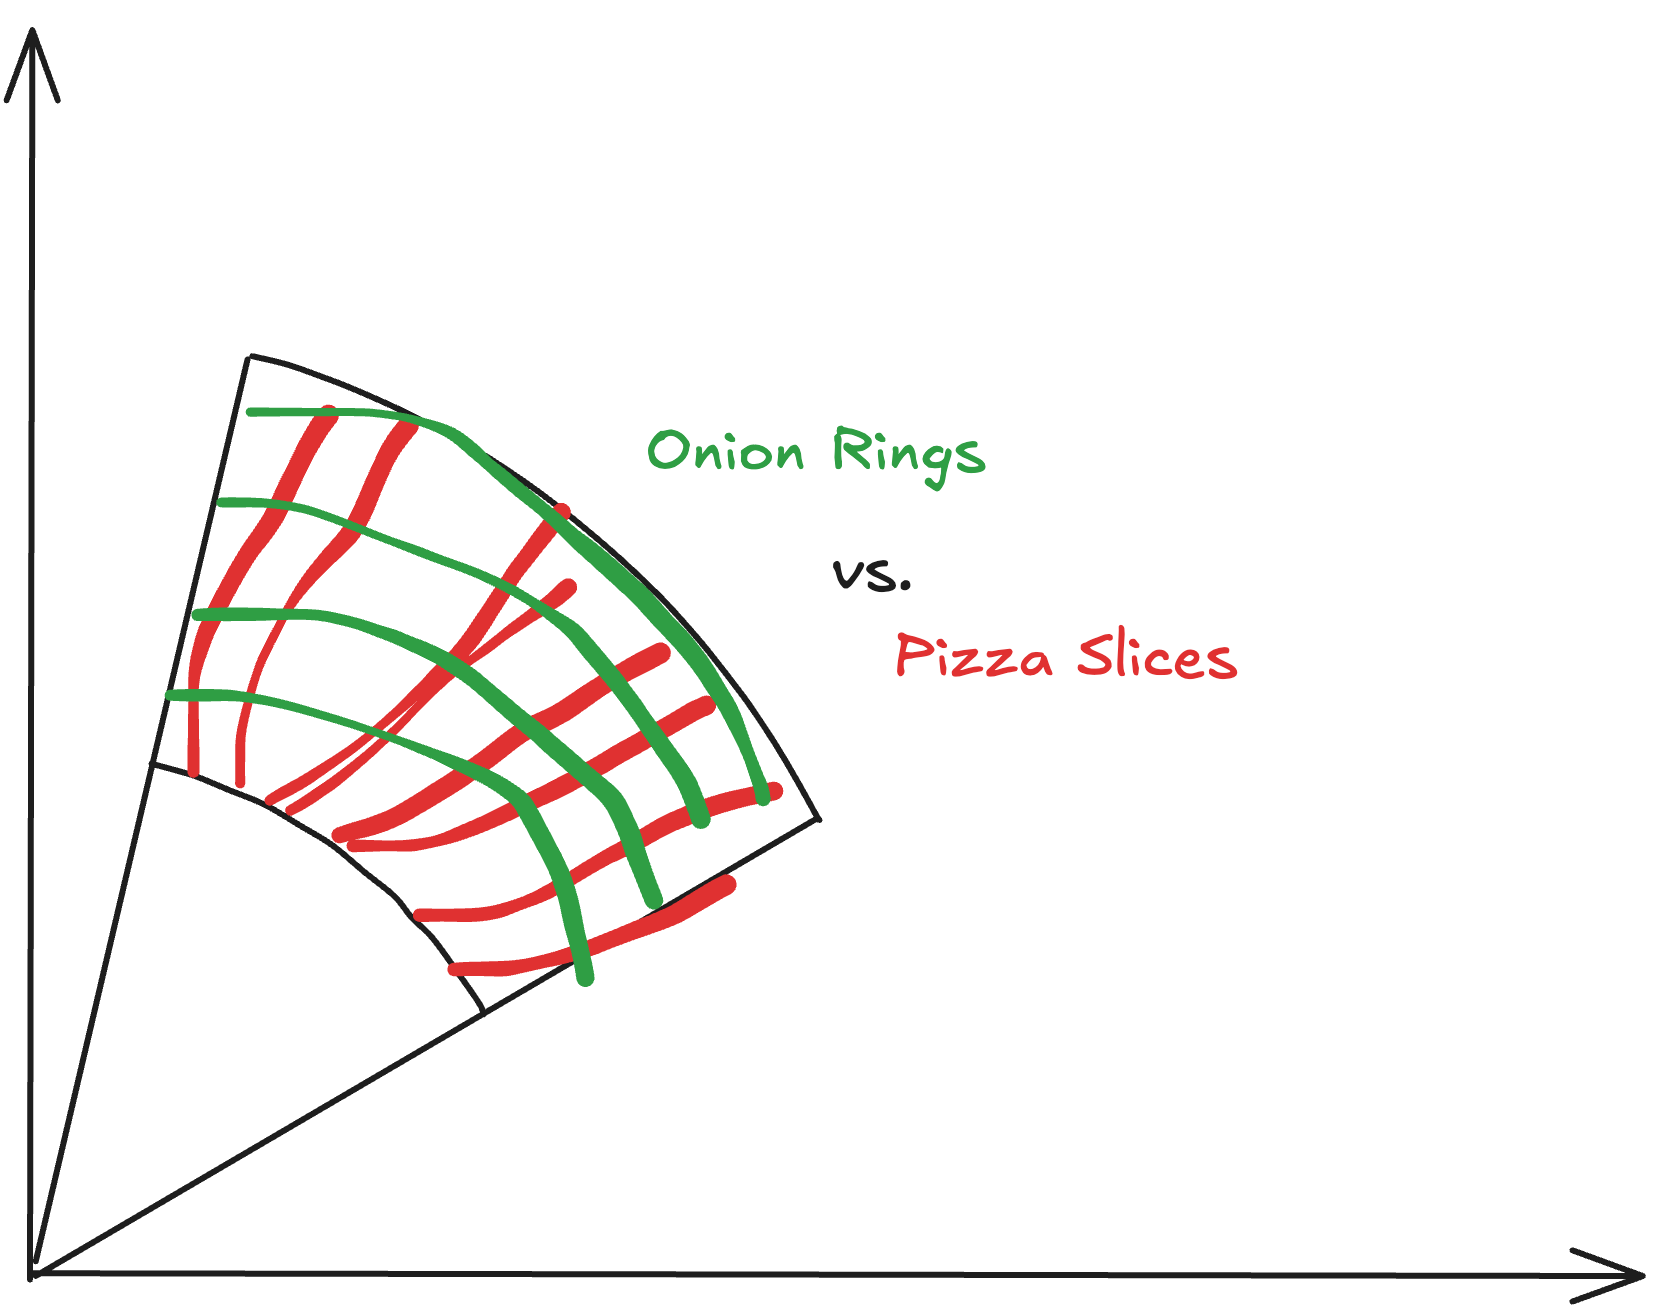
\includegraphics[width=0.3\textwidth]{figures/PizzavsOnions.png}
\end{figure}

$$x = r \cos \theta$$
$$y = r \sin \theta$$

$$\iint f(x, y) \delta A = \iint f(r\cos\theta, r\sin\theta) r \delta r \delta \theta$$

Some restrictions

\begin{itemize}
    \item $0 \leq \theta < 2\pi$
    \item $r$ has to be positive.
\end{itemize}

\section{Triple Integrals}

\subsection{Triple Integrals in Rectangular Form}

\begin{figure}[H]
    \centering
    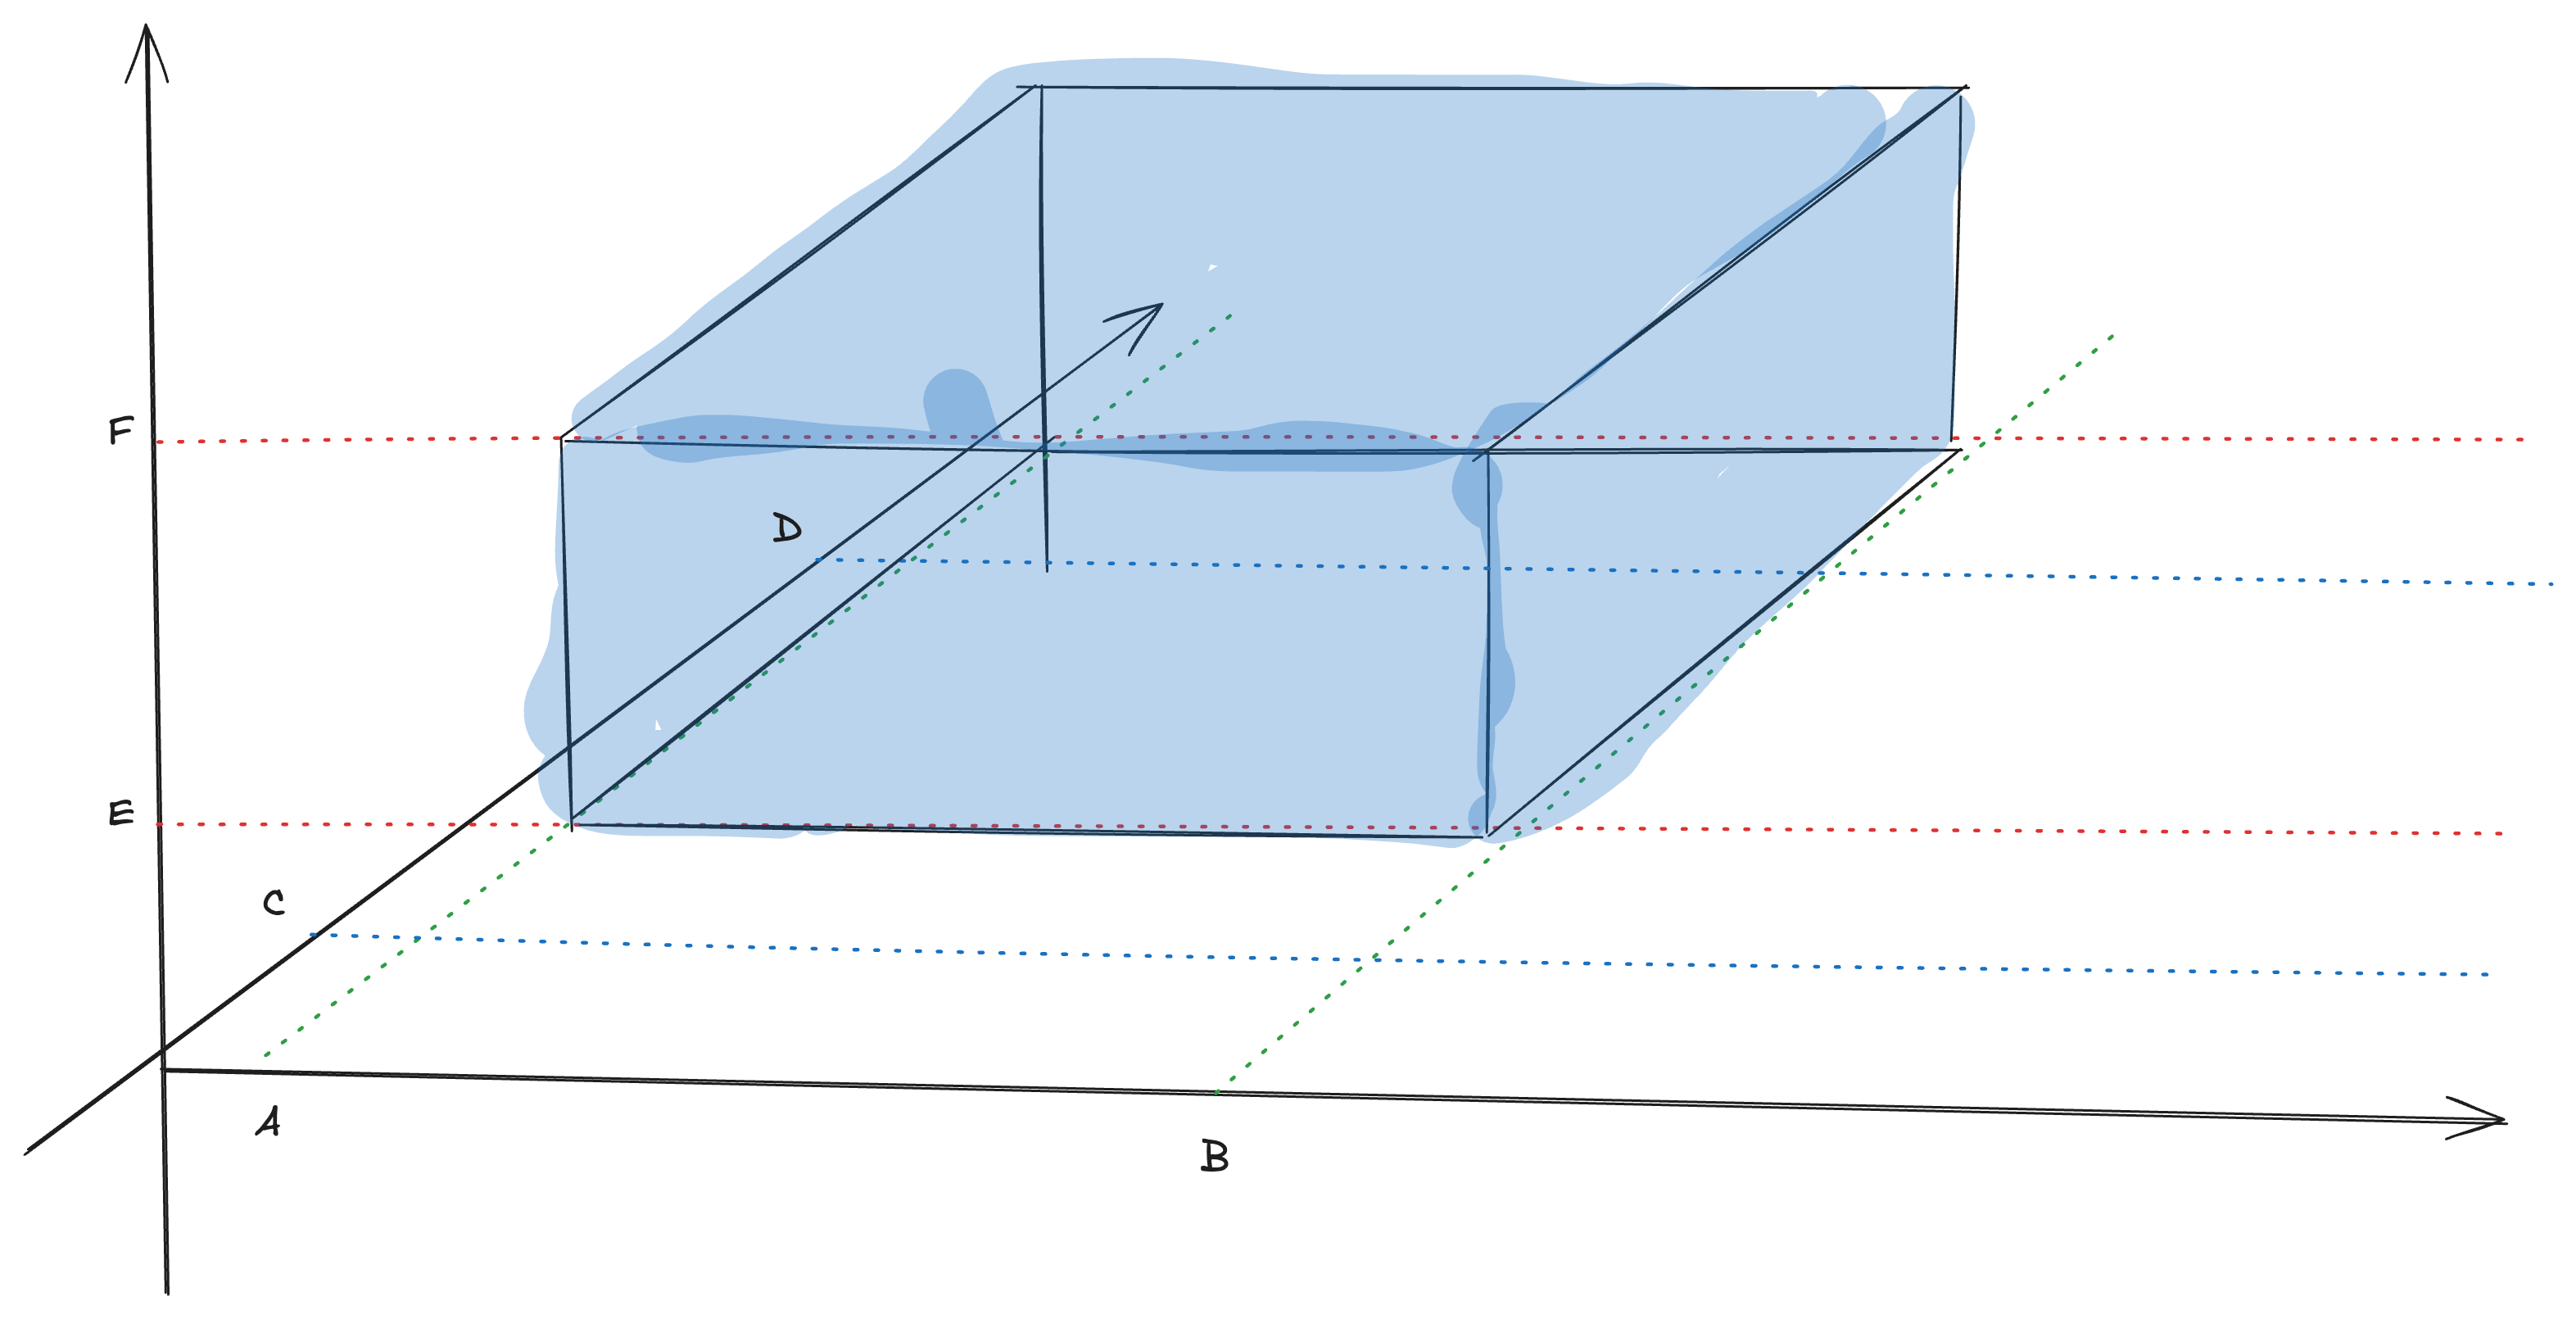
\includegraphics[width=0.5\textwidth]{figures/Rectangle.png}
    \caption{Three Dimensional Object}
\end{figure}

To integrate over three dimensional object, one can use triple integrals.

$$\iiint_E f(x, y, z)$$

Think about it as little cubes, with $$\lim_{m, n, l \to \infty} \Sigma_{k=1}^l \Sigma_{j = 1}^{m} \Sigma_{i = 1}^n f(y_{ijk}^*, y_{ijk}^*, z_{ijk}^*) \Delta x \Delta y \Delta z$$

\subsubsection{Three Type of Regions of Space}

\textbf{Type 1}

\begin{figure}[H]
    \centering
    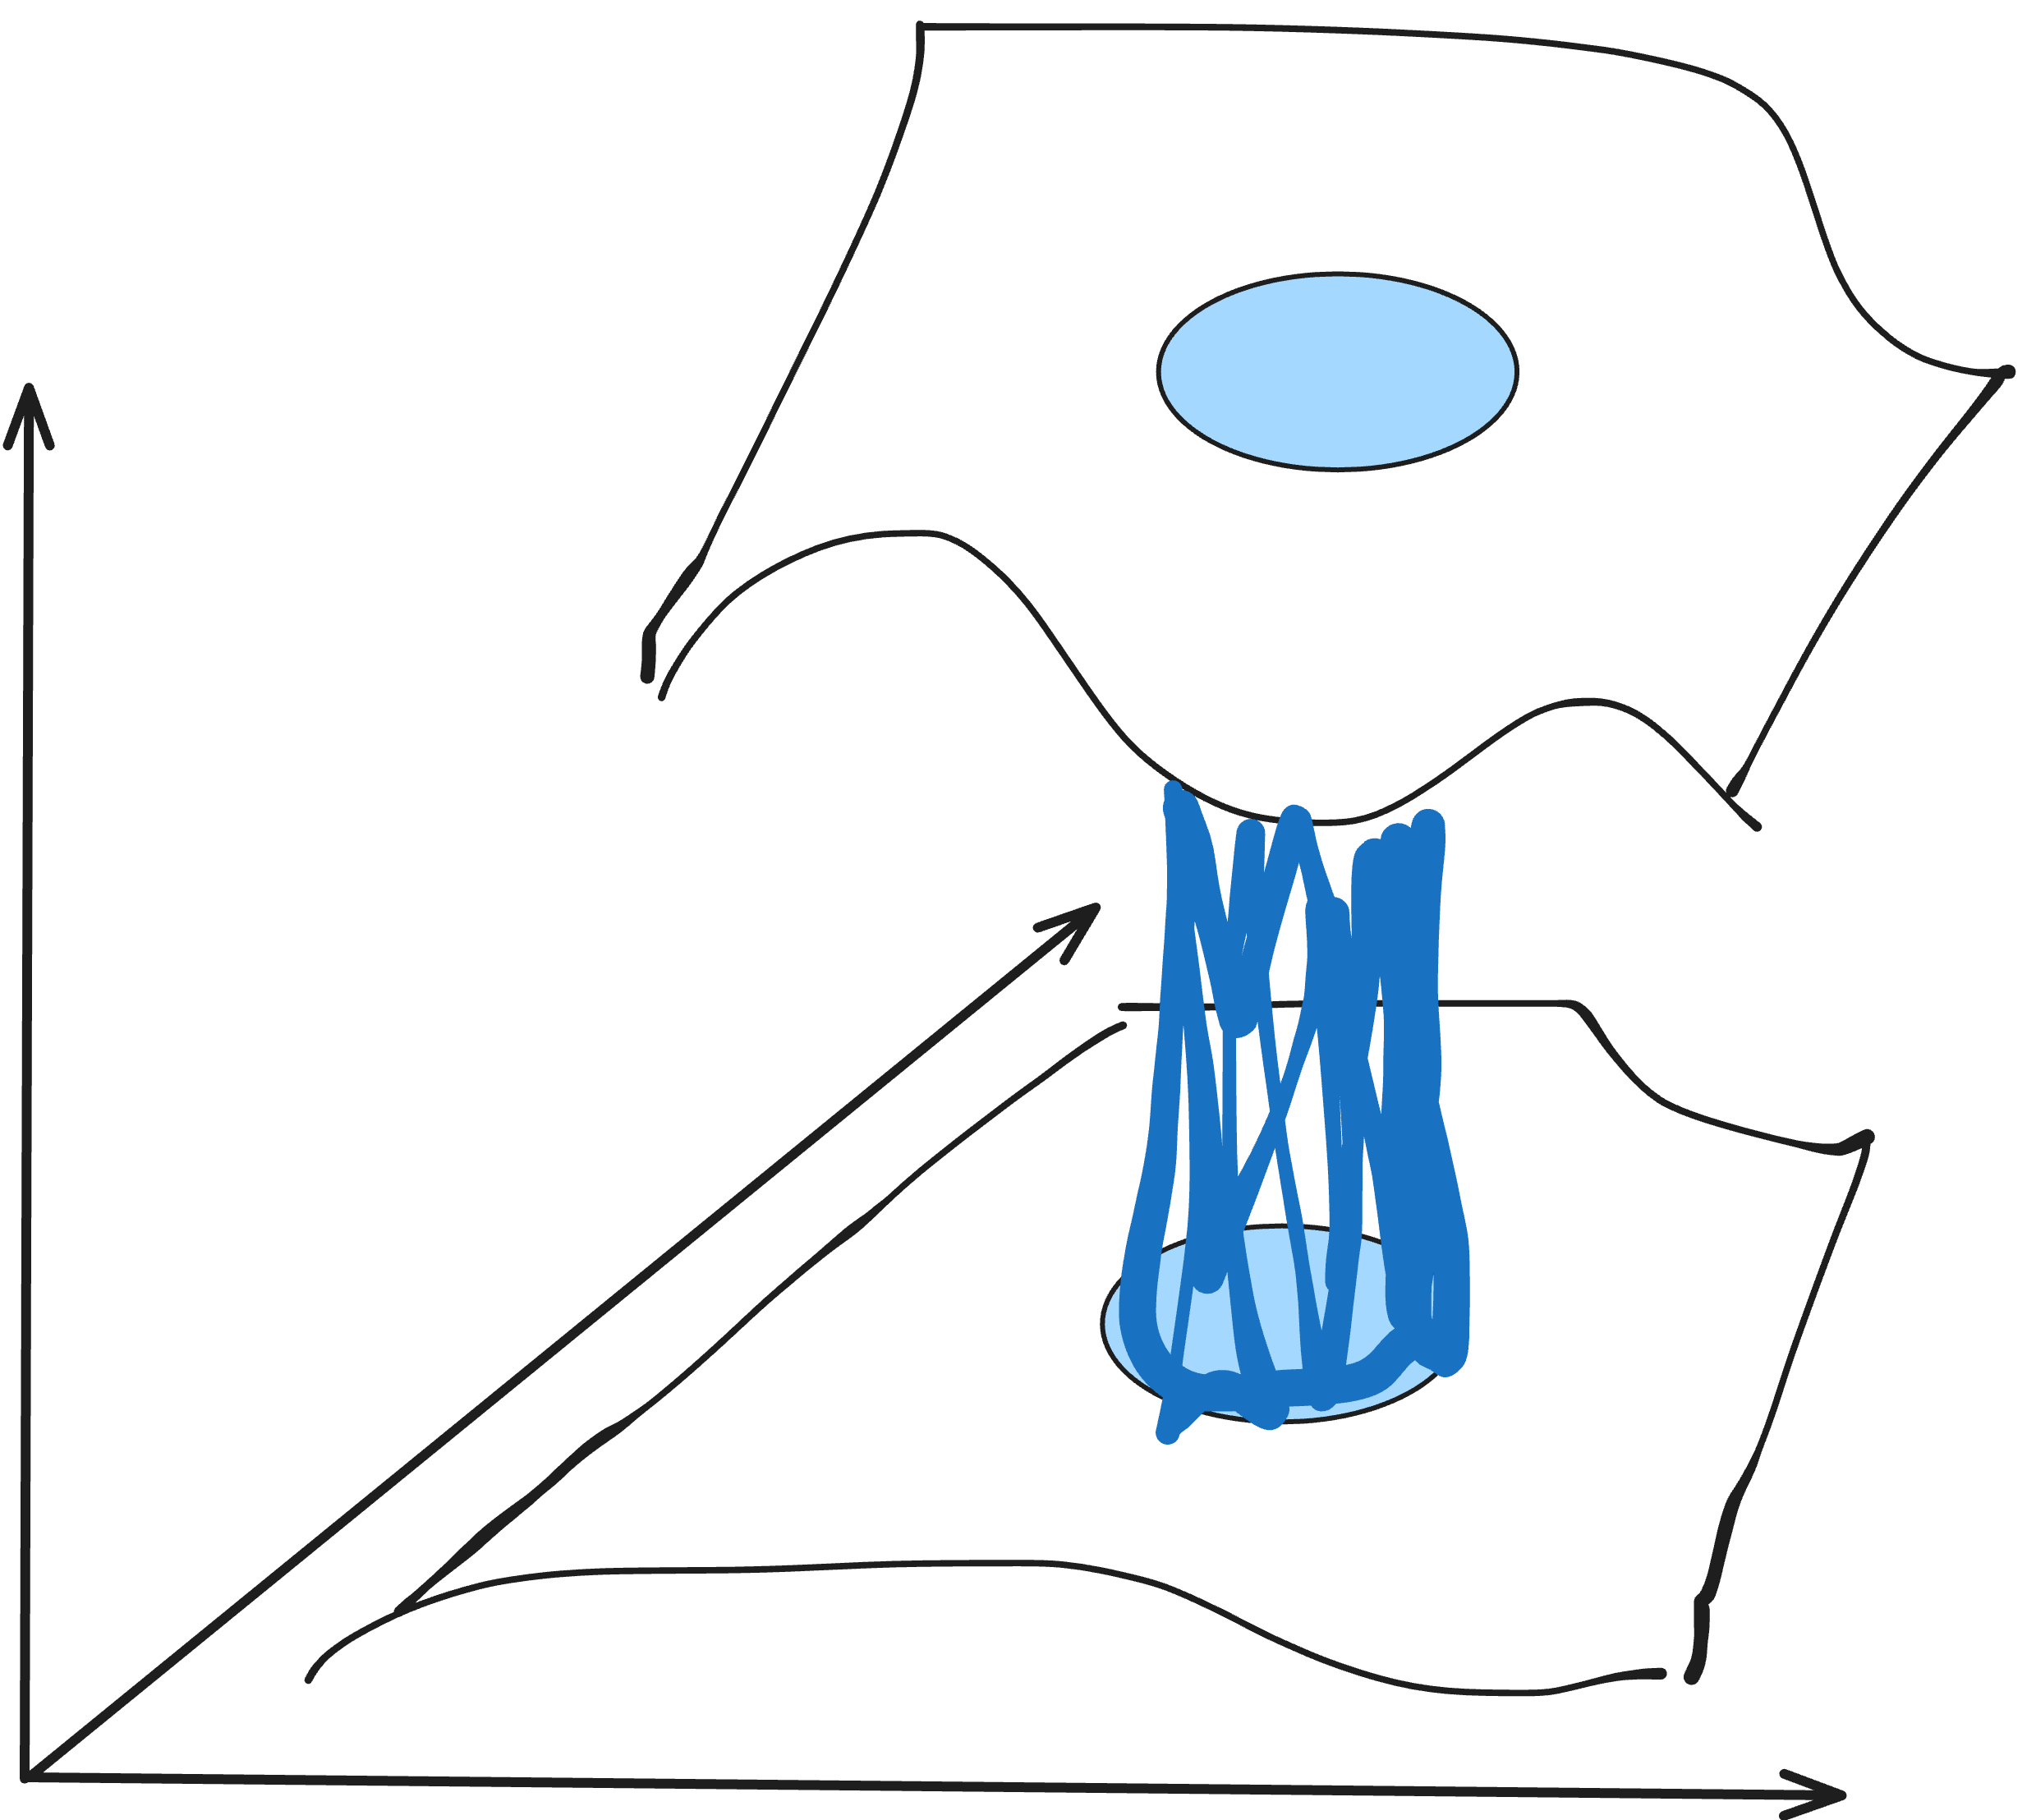
\includegraphics[width=0.3\textwidth]{figures/RegionISpace.png}
    \caption{Example of a type 1 surface}
\end{figure}

$$\iiint_E f(x, y, z) \delta V = \iint_D \int_{g_2(x, y)}^{g_1(x, y)} g_2 - g_1 \delta z \delta A$$

\textbf{Type 2}

\begin{figure}[H]
    \centering
    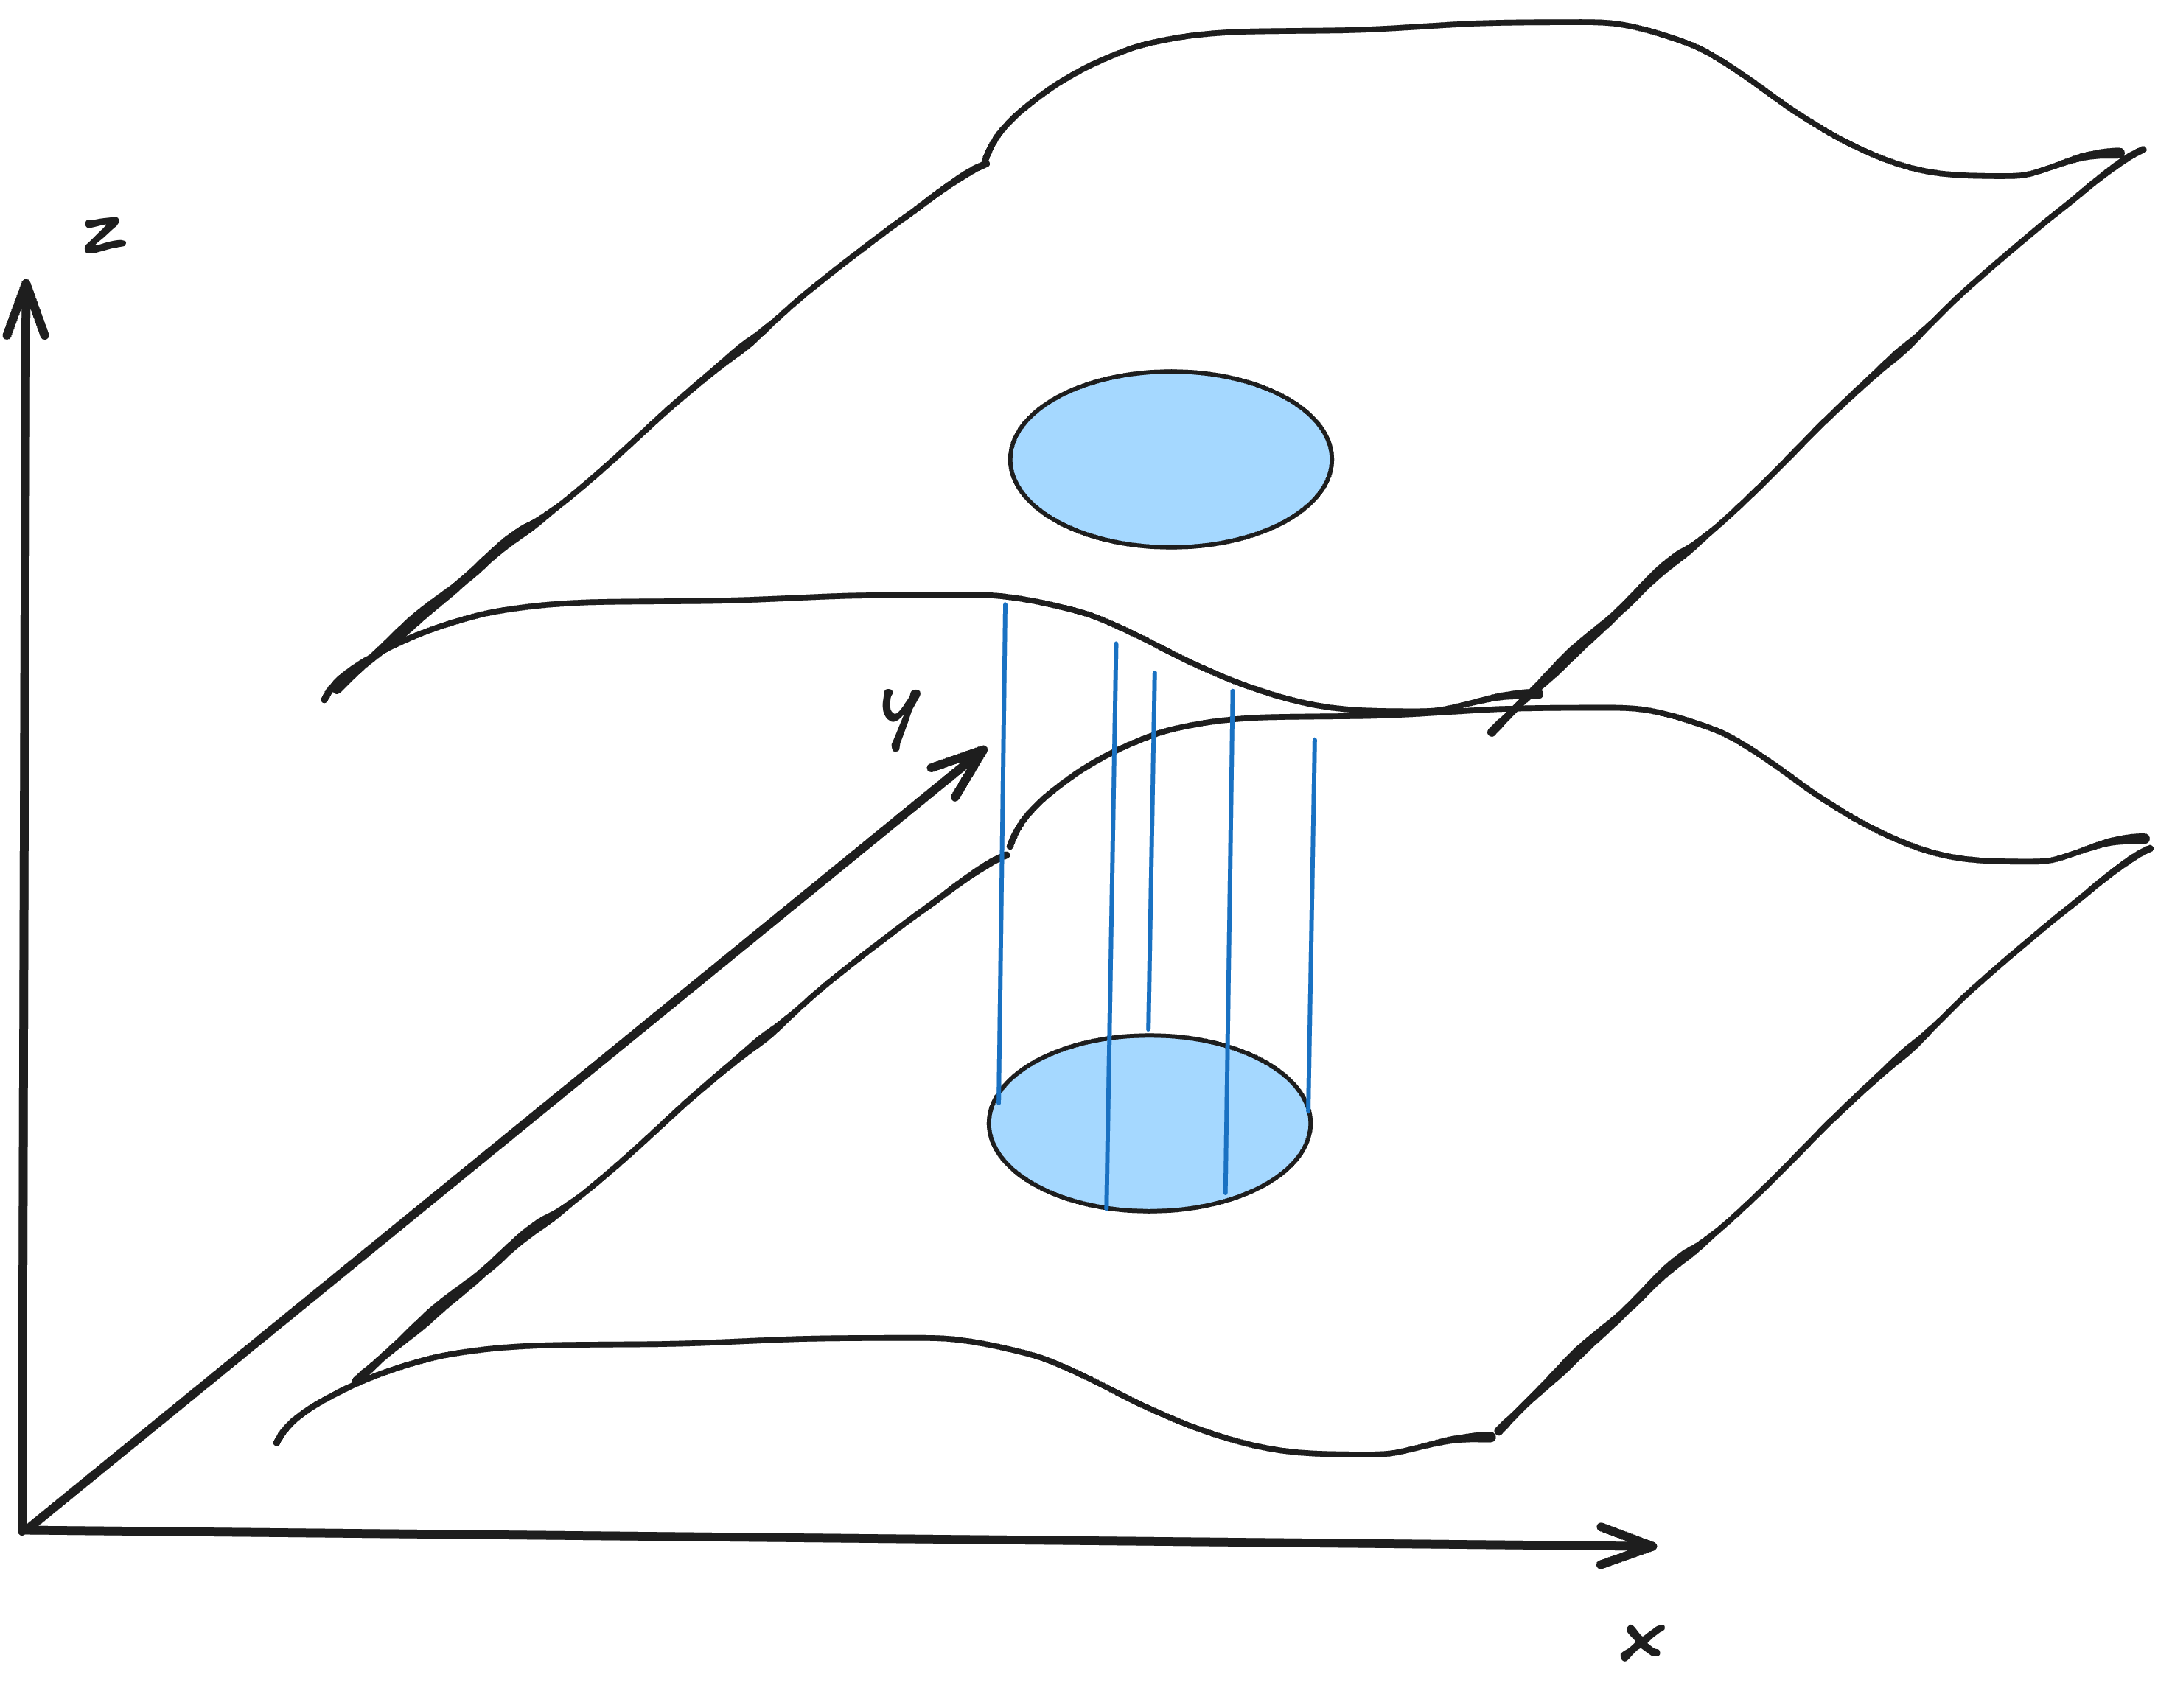
\includegraphics[width=0.3\textwidth]{figures/type2surfaces.png}
    \caption{Example of a type 2 surface}
\end{figure}

$$\iiint_E f(x, y, z) \delta V = \iint_D \int_{h_2(x, y)}^{h_1(x, y)} h_2 - h_1 \delta y \delta A$$

\textbf{Type 3}

\begin{figure}[H]
    \centering
    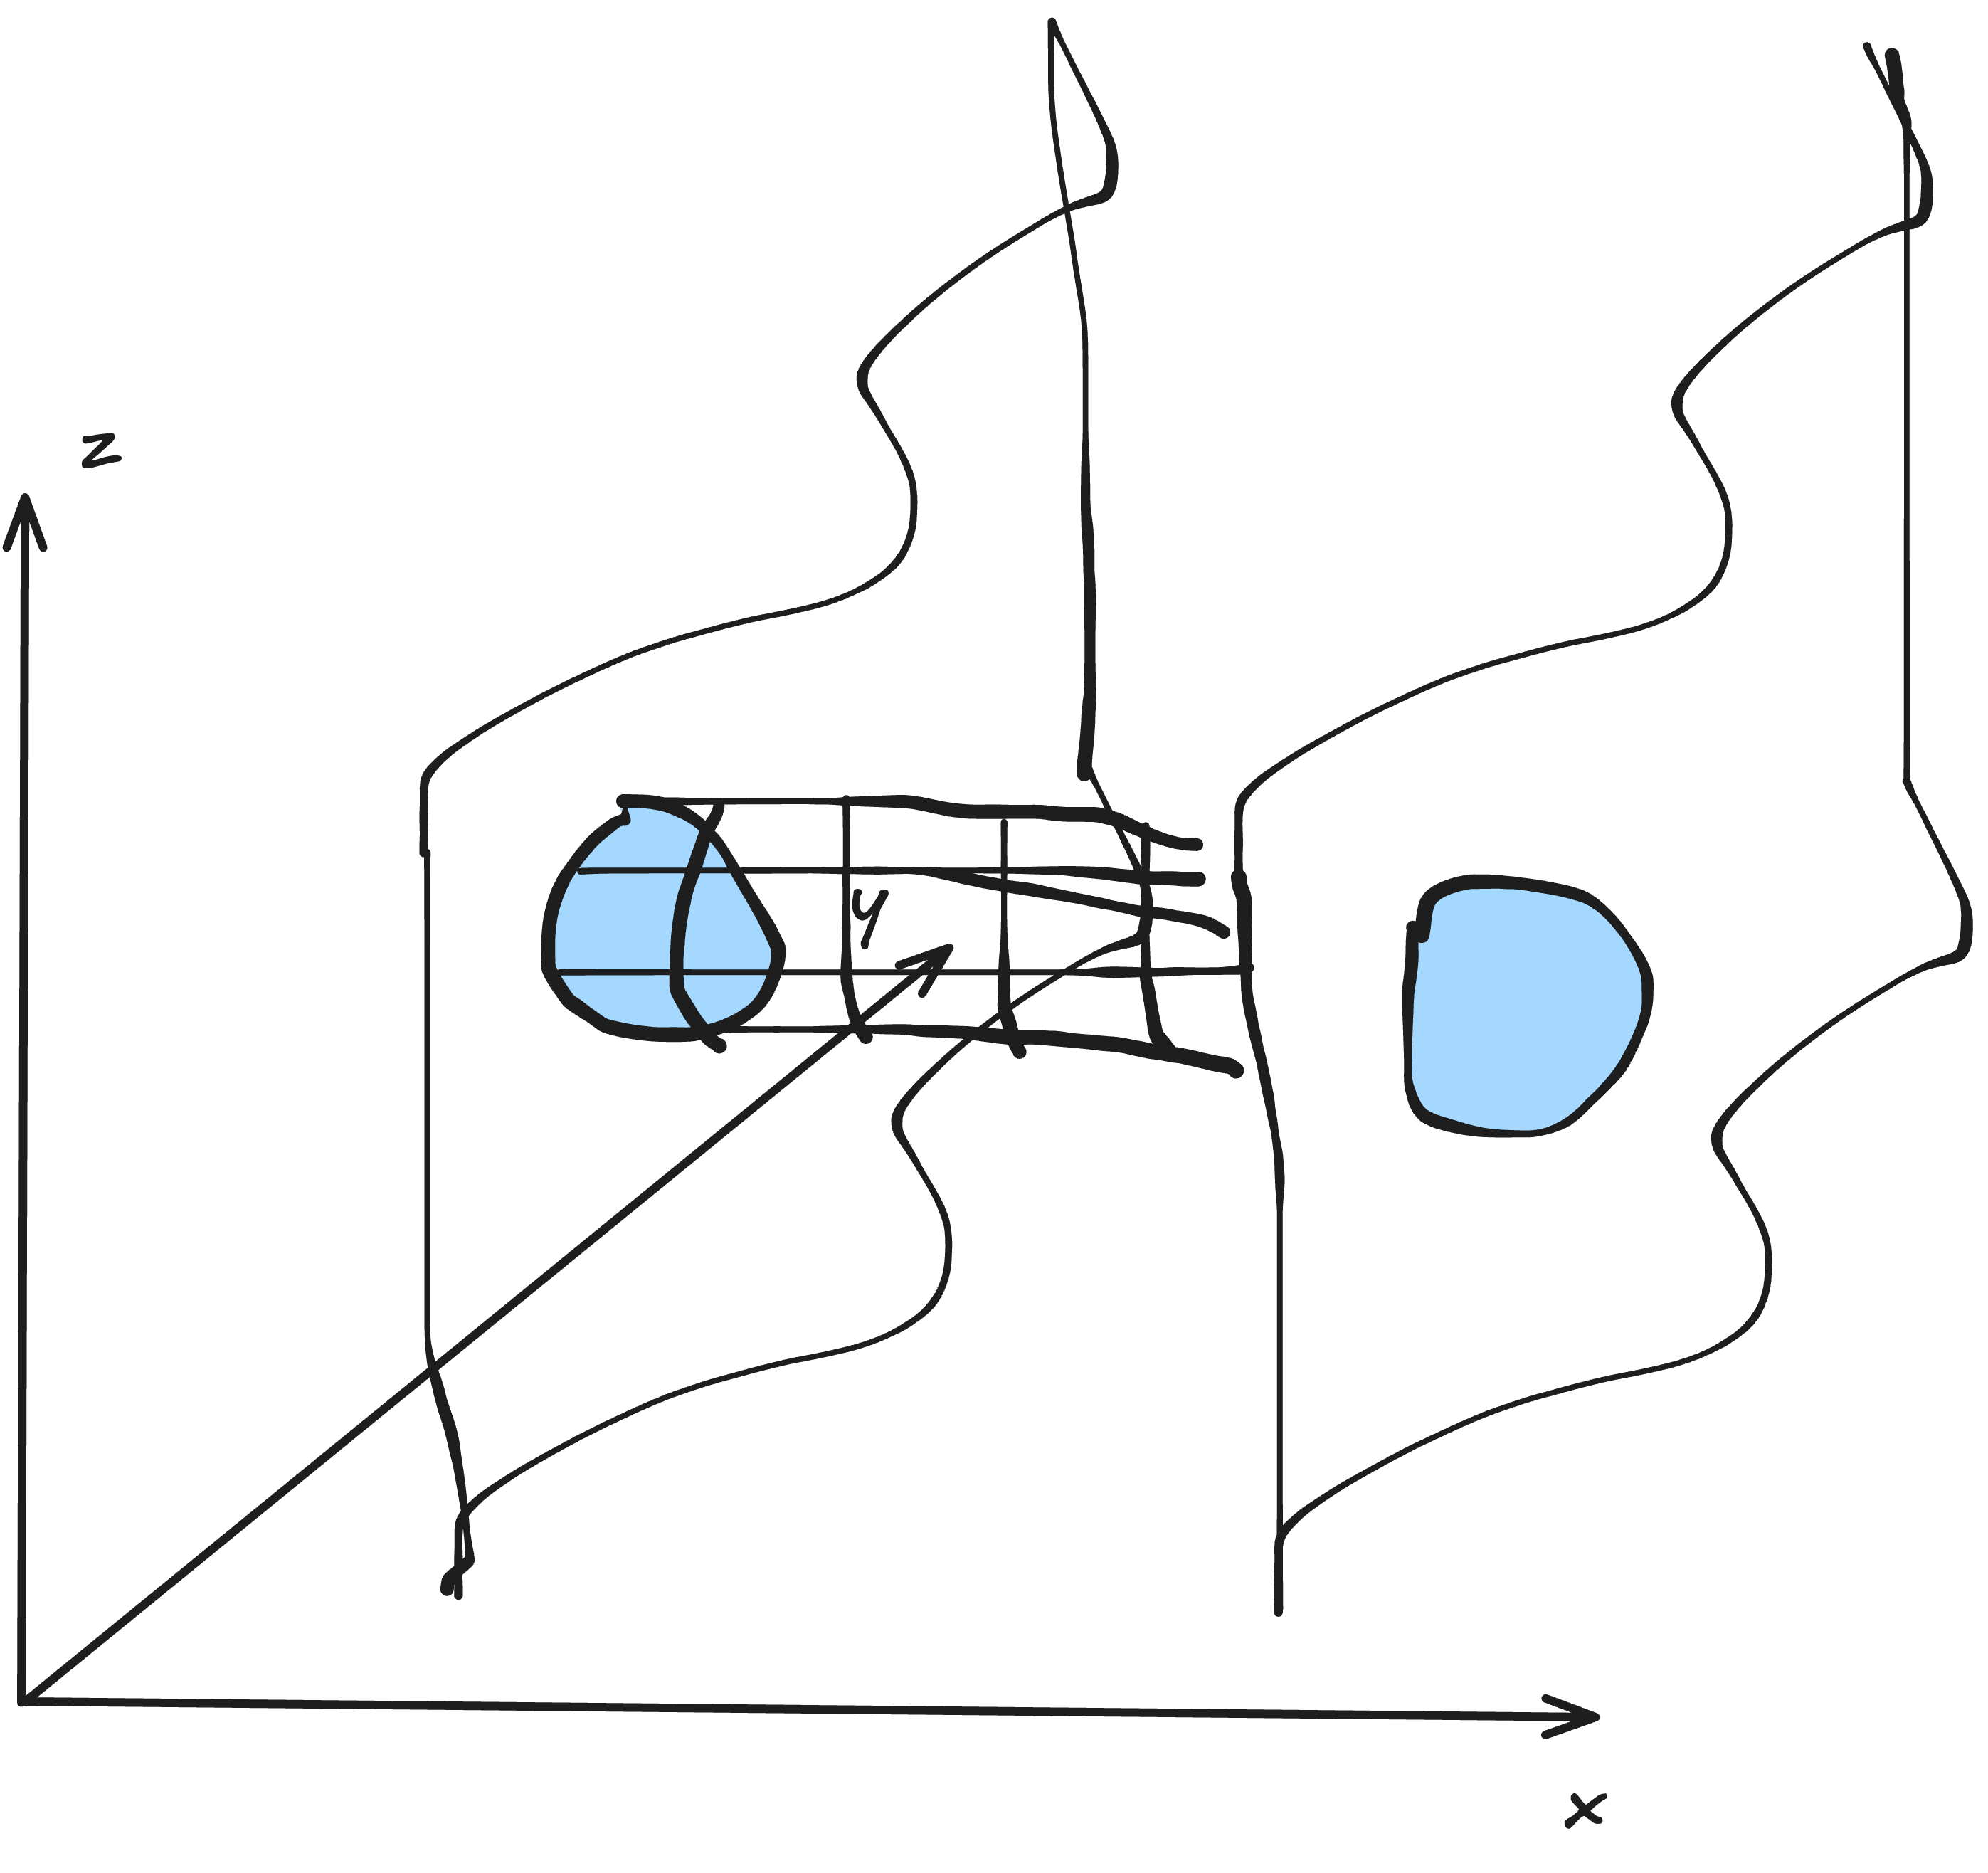
\includegraphics[width=0.3\textwidth]{figures/type3surfaces.png}
    \caption{Example of a type 3 surface}
\end{figure}

$$\iiint_E f(x, y, z) \delta V = \iint_D \int_{k_2(x, y)}^{k_1(x, y)} k_2 - k_1 \delta x \delta A$$


\subsection{Triple Integrals in Cylindrical Form}

Spherical coordinates basically add an additional z dimension to the normal polar integrals.

\begin{figure}[H]
    \centering
    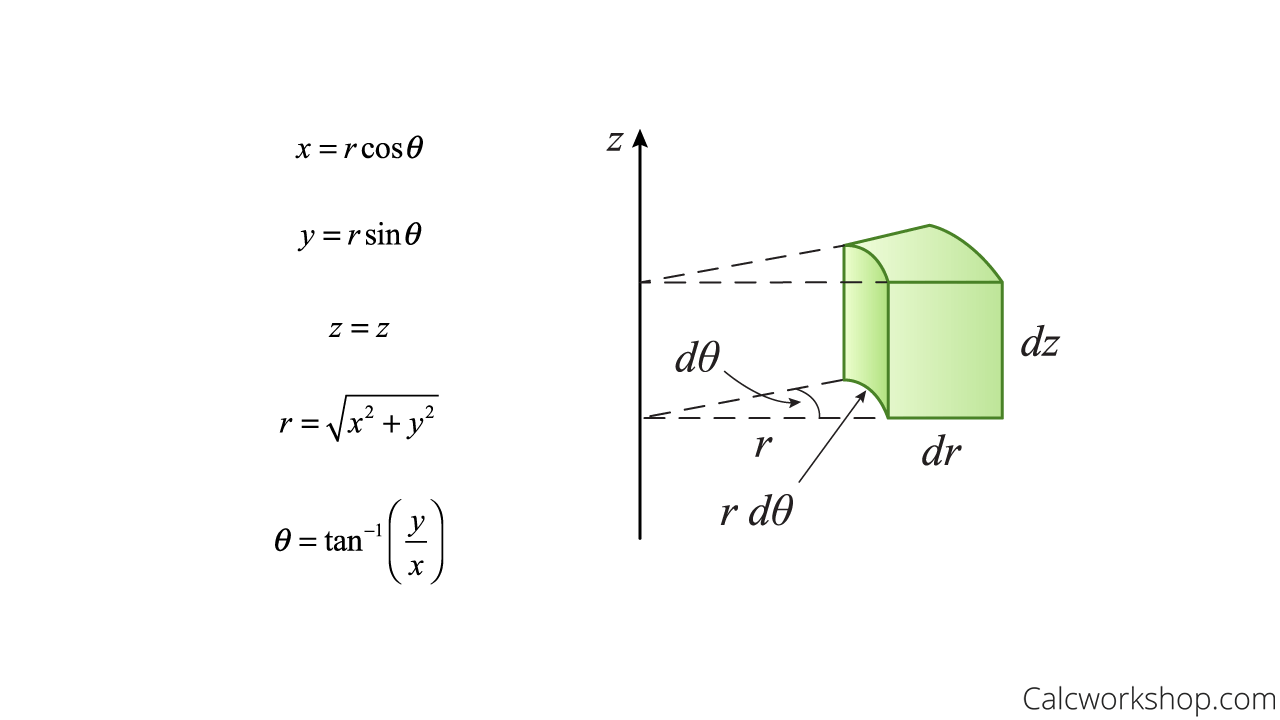
\includegraphics[width=0.4\textwidth]{figures/cylindrical.png}
    \caption{Example of cylindrical coordinates}
\end{figure}

To convert between cylindrical and rectantular, you just have to add a z:\\
\textbf{(cylindrical to rectangular)}

$$\text{Given } P(x, y, z) \text{ and } P(r,\theta, z) \text{ represent the same point},\quad x = r \cos\theta,\quad y = r sin \theta, \quad z = z$$

\textbf{(rectangular to cylindrical)}

$$r^2=x^2+y^2,\quad \tan \theta = \frac{y}{x}, \quad z = z$$

\subsection{Triple Integrals in Spherical Form}

Sphericals turn the 2D pizza into a 3D sphere of greatness.

\begin{figure}[H]
    \centering
    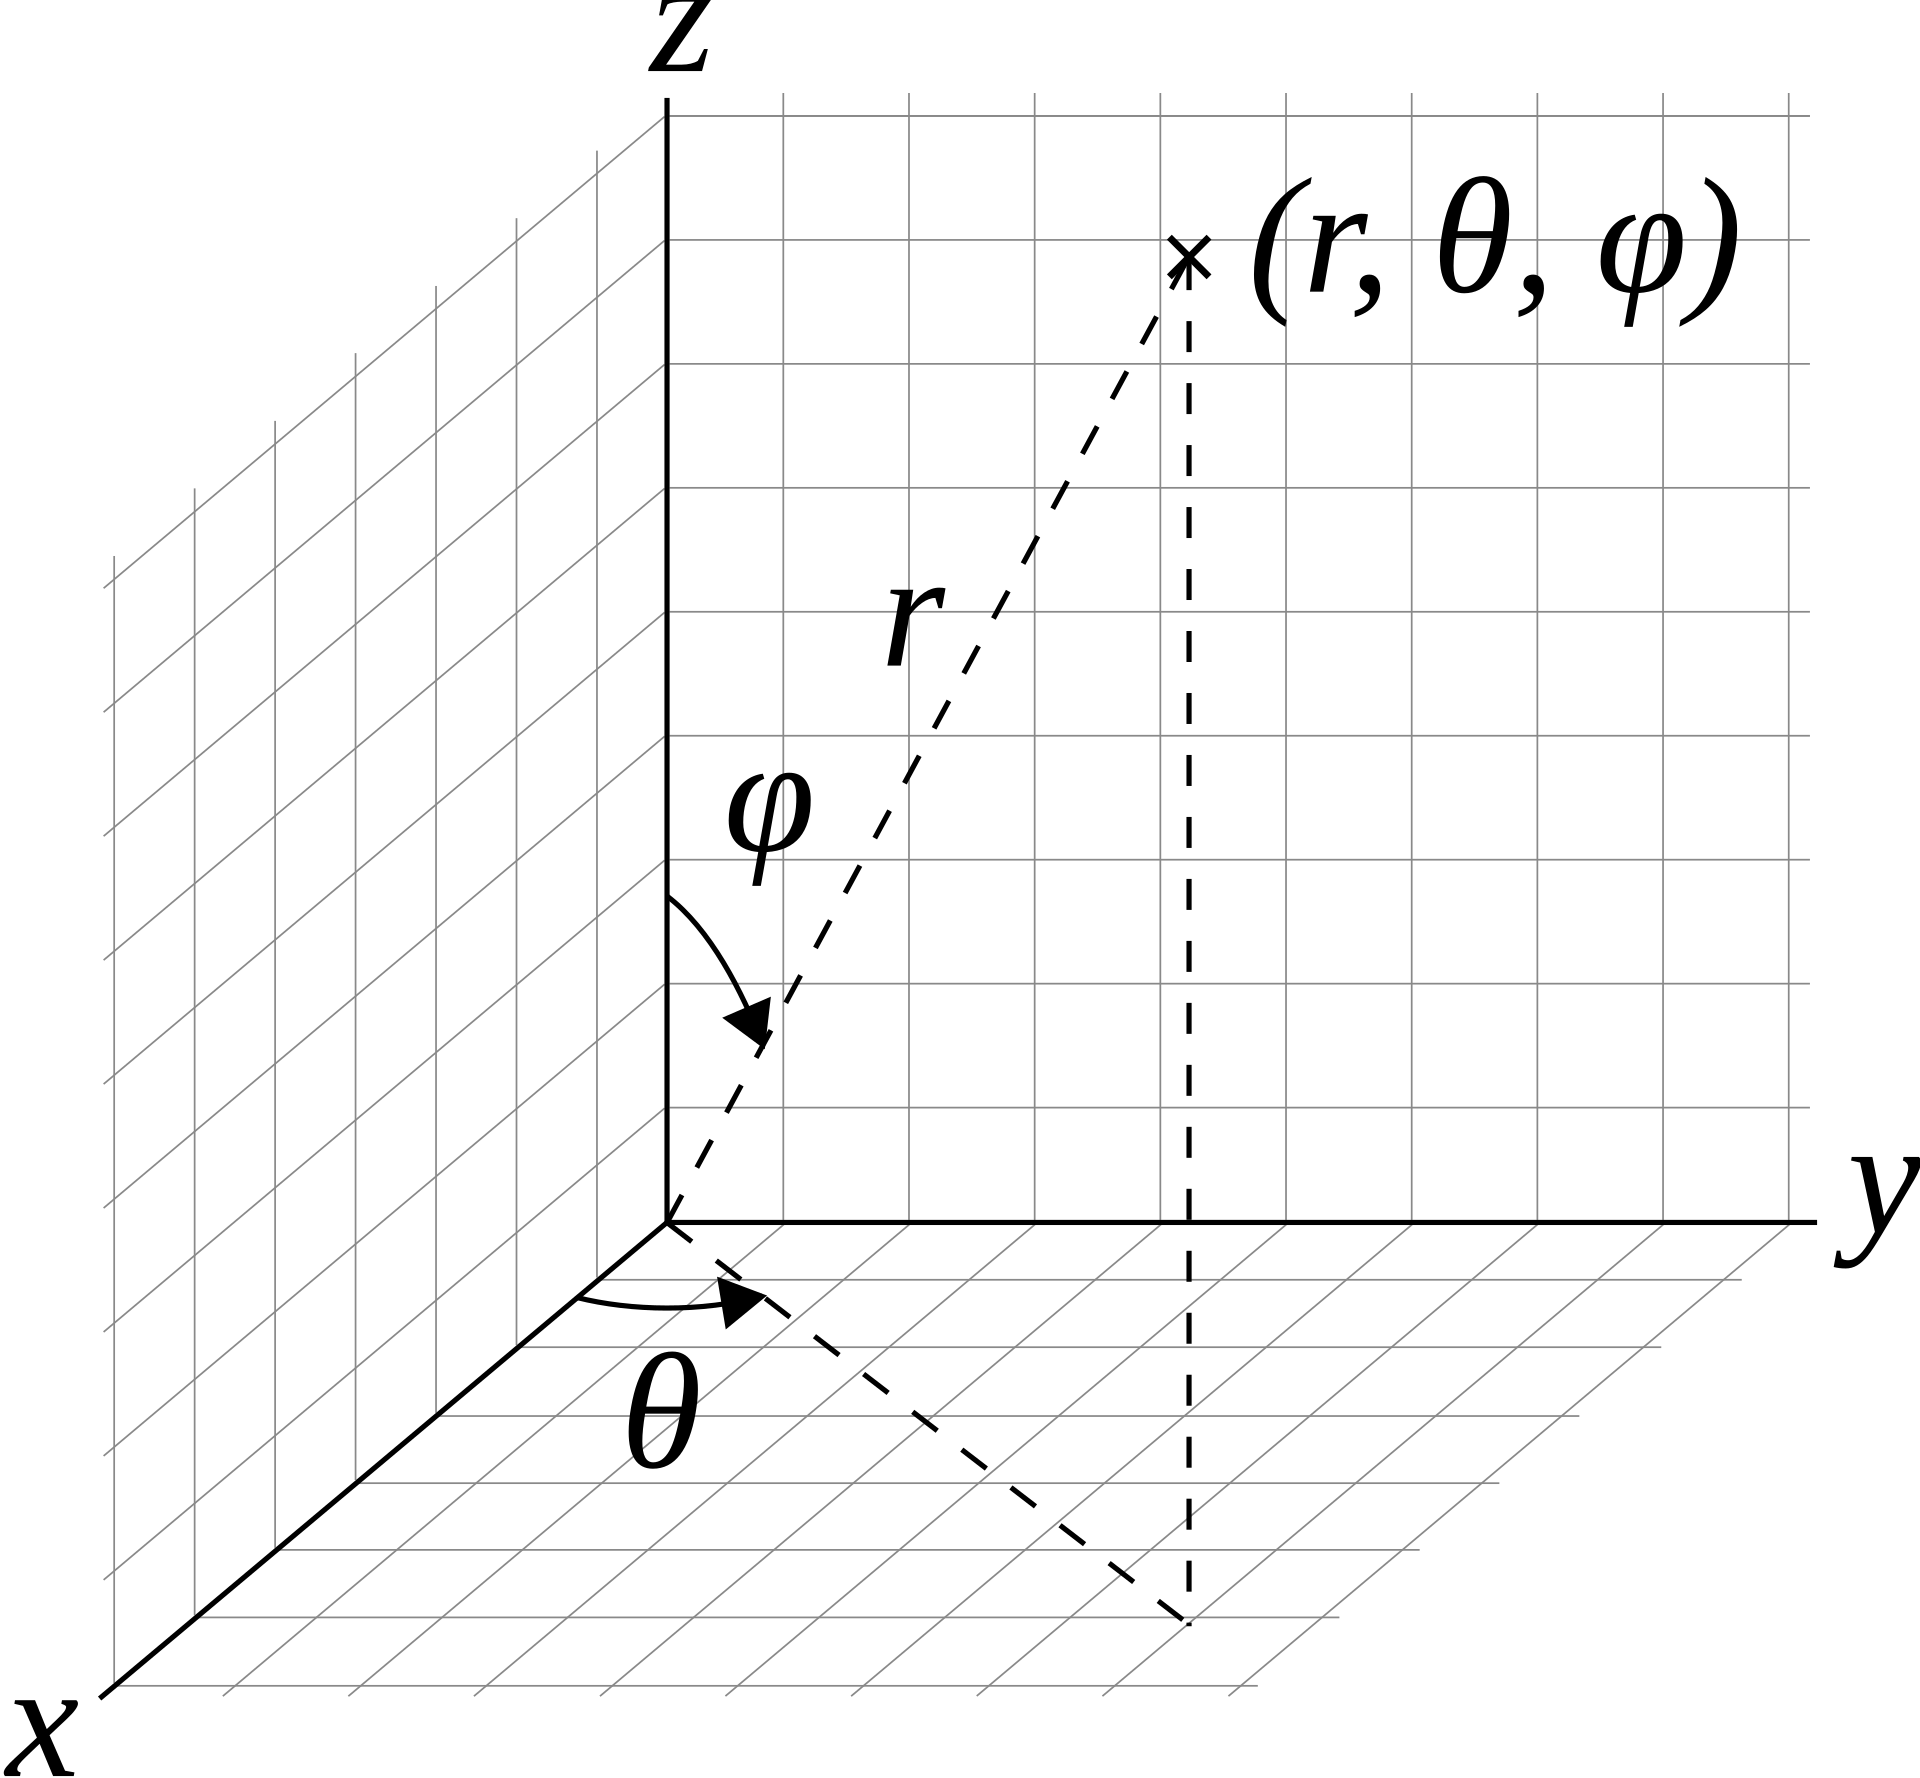
\includegraphics[width=0.3\textwidth]{figures/spherical_coordinates.png}
    \caption{Example of spherical coordinates}
\end{figure}

If $P(x, y, z)$ and $P(r, \theta, \phi)$ represent the same point in rectangular and spherical coordinates, then \\
\textbf{(spherical to rectangular)}

$$x = r\cos\theta\sin\phi, \quad y = r\sin\theta\sin\phi, \quad z = r\cos\phi$$

\textbf{(rectangular to cylindrical)}

$$\rho^2 = x^2 + y^2 + z^2, \quad \tan \theta = \frac{y}{x}, \quad \cos \phi = \frac{\sqrt{x^2 + y^2}}{z}$$

\section{Changing the Order of Integration}

To change the bounds of an integral, all you do is to try to visualize the graph of the function, and then change the integrands to that.\\
\textbf{Example}
$$\int_{0}^{1}\int_{0}^{7} \delta x \delta y = \int_{0}^{1} \int_{x}^{1} f(x, y) \delta y \delta x$$



\end{document}